% Provenance (never printed): see sources/outline_sources.md (Year 1: crystal
% chemistry of minerals, silicates, solid solutions, mineral formulas, the main
% rock-forming minerals). Olivine curves in figdata/bachelor-1/solid_solution.py;
% the olivine analysis of the problem is invented (Fo about 82); exercise and
% problem values in the Book 3 scratch calculator calc/ch07.py.
\chapter{Minerais formadores de rochas}\label{ch:b1:rock-forming-minerals}

Uma bancada de granito mostra três ou quatro tipos de grão: quartzo cinzento e vítreo, \omterm{def:b1:rock-forming-minerals:groups}{feldspato} rosado ou branco, lamelas de \omterm{def:b1:rock-forming-minerals:groups}{mica} preta. Uma areia de praia é quase toda quartzo. Os pequenos cristais verdes espalhados em um basalto são \omterm{def:b1:rock-forming-minerals:groups}{olivina}, e o mesmo \omterm{def:b1:rock-forming-minerals:mineral}{mineral}, numa composição um pouco diferente, forma a maior parte do manto superior. Um punhado de \omterm{def:b1:rock-forming-minerals:mineral}{minerais} constrói quase todas as rochas, e quase todos são silicatos: oxigênio e silício, os dois elementos mais abundantes da crosta, unidos em tetraedros que se ligam de algumas maneiras simples. Este capítulo explica como essa ligação fixa a fórmula e o hábito de um silicato, como um elemento substitui outro num cristal, de modo que um \omterm{def:b1:rock-forming-minerals:mineral}{mineral} é uma faixa de composições e não uma composição única, como uma análise química se torna uma fórmula e quais são os principais \omterm{def:b1:rock-forming-minerals:mineral}{minerais} formadores de rochas. Ele termina com uma \omterm{def:b1:rock-forming-minerals:groups}{olivina} de um basalto, analisada, recalculada e pesada.

\begin{recall}
Um cristal é um sólido cujos átomos se repetem em uma rede; a célula unitária é a menor caixa que se repete, e o número de coordenação de um íon conta os seus vizinhos mais próximos de carga oposta (química, no volume do primeiro ano). Os raios iônicos dependem da carga e da coordenação. Um \omterm{def:b1:rock-forming-minerals:mineral}{mineral} é identificado na mão pelo seu hábito, pela clivagem, pela dureza e pelo brilho (Livro 2, 11º ano). A quantidade de substância conta-se em mols, e a massa molar é a massa de um mol (química).
\end{recall}

\section{O que é um mineral}

\begin{definition}[Mineral]\label{def:b1:rock-forming-minerals:mineral}
Um \emph{mineral}\index{mineral} é um sólido de ocorrência natural, com estrutura cristalina definida e composição química que é fixa ou varia dentro de limites definidos. Quase todos os minerais são inorgânicos.
\end{definition}

Uma rocha, ao contrário, é um agregado de grãos de um ou de vários \omterm{def:b1:rock-forming-minerals:mineral}{minerais} (ou de vidro): o granito é quartzo, \omterm{def:b1:rock-forming-minerals:groups}{feldspatos} e \omterm{def:b1:rock-forming-minerals:groups}{mica}; o calcário é sobretudo calcita. As duas metades da definição são independentes. O vidro de janela tem a composição de um silicato, mas nenhuma estrutura cristalina: não é um \omterm{def:b1:rock-forming-minerals:mineral}{mineral}, nem o vidro de uma lava resfriada rapidamente. Inversamente, a mesma composição pode cristalizar em várias estruturas, e cada estrutura é um \omterm{def:b1:rock-forming-minerals:mineral}{mineral} diferente.

\begin{definition}[Polimorfo]\label{def:b1:rock-forming-minerals:polymorph}
Dois \omterm{def:b1:rock-forming-minerals:mineral}{minerais} são \emph{polimorfos}\index{polimorfo} um do outro quando têm a mesma composição química e estruturas cristalinas diferentes.
\end{definition}

O carbono cristaliza como grafita, uma pilha de folhas de hexágonos com densidade de \qty{2.16}{g.cm^{-3}}, e como diamante, uma estrutura em que cada átomo tem quatro vizinhos, com densidade de \qty{3.51}{g.cm^{-3}}. O carbonato de cálcio é calcita (\qty{2.71}{g.cm^{-3}}) ou aragonita (\qty{2.93}{g.cm^{-3}}); a sílica é quartzo (\qty{2.65}{g.cm^{-3}}) ou coesita (\qty{2.93}{g.cm^{-3}}); \ce{Al2SiO5} é cianita (\qty{3.61}{g.cm^{-3}}), andalusita (\qty{3.15}{g.cm^{-3}}) ou silimanita (\qty{3.24}{g.cm^{-3}}).
% ledger: webmineral:polymorphs, hom:calcite, hom:quartz
Em cada par, o \omterm{def:b1:rock-forming-minerals:polymorph}{polimorfo} mais denso é o que se forma sob maior pressão: a uma dada temperatura, aumentar a pressão favorece o estado de menor volume (química, o deslocamento de um equilíbrio). Diamante em um kimberlito e coesita em uma rocha atingida por um meteorito registram, portanto, pressões encontradas apenas no fundo do manto ou em um impacto. Os três \omterm{def:b1:rock-forming-minerals:polymorph}{polimorfos} de \ce{Al2SiO5}, cujos campos de estabilidade dividem entre si o plano pressão--temperatura, servem para ler as condições do metamorfismo (no Livro 4).

\section{O tetraedro de silicato e suas ligações}

Em todo silicato comum, cada átomo de silício fica no centro de quatro átomos de oxigênio dispostos nos vértices de um tetraedro regular: a unidade \ce{SiO4} relembrada da química. O íon silício é pequeno (\qty{0.26}{\angstrom} em coordenação quádrupla) e o íon óxido é grande, de modo que quatro oxigênios cabem em torno dele e não mais; a ligação silício--oxigênio é forte e parcialmente covalente. Uma unidade isolada carrega a carga $4 - 4\times2 = -4$.
% ledger: shannon:radii
Os tetraedros podem ficar isolados, com a carga equilibrada por cátions metálicos entre eles, ou compartilhar vértices: um oxigênio comum a dois tetraedros é um \emph{oxigênio em ponte}. Dois tetraedros nunca compartilham uma aresta ou uma face, o que aproximaria demais dois silícios. Os silicatos são classificados pelo número de vértices que cada tetraedro compartilha (\cref{def:b1:rock-forming-minerals:silicate-classes}).

\begin{omfigure}
\tikzset{
  tup/.pic={\filldraw[fill=omLithLime, draw=black, line join=round] (0,0) -- (1,0) -- (0.5,0.866) -- cycle;
            \fill[omThm] (0.5,0.2887) circle (0.11);},
  tdn/.pic={\filldraw[fill=omLithLime, draw=black, line join=round] (0,0) -- (1,0) -- (0.5,-0.866) -- cycle;
            \fill[omThm] (0.5,-0.2887) circle (0.11);},
  linkpanel/.style={x=0.45cm, y=0.45cm, baseline=(current bounding box.south)}}
\setlength{\tabcolsep}{4pt}
\begin{tabular}{cccc}
% (a) the tetrahedron in perspective
\begin{tikzpicture}[linkpanel]
  \useasboundingbox (-1.2,-1.0) rectangle (6.0,4.4);
  \coordinate (T) at (2.2,3.7); \coordinate (L) at (0.3,0.5); \coordinate (R) at (4.1,0.1);
  \coordinate (B) at (3.3,2.1); \coordinate (C) at (2.475,1.6);
  \draw[densely dashed, gray] (L) -- (B) -- (R) (B) -- (T);
  \shade[ball color=omLithShale] (B) circle (0.42);
  \draw[gray] (C) -- (T) (C) -- (L) (C) -- (R) (C) -- (B);
  \shade[ball color=omThm!70] (C) circle (0.24);
  \draw[thick, line join=round] (T) -- (L) -- (R) -- cycle;
  \foreach \p in {T,L,R} \shade[ball color=omLithShale] (\p) circle (0.42);
  \node[right] at (4.5,0.1) {\scriptsize O};
  \node[right] at (2.6,3.8) {\scriptsize O};
  \draw[omThm] (C) -- (4.6,2.2) node[right] {\scriptsize Si};
\end{tikzpicture} &
% (b) nesosilicate: isolated tetrahedra
\begin{tikzpicture}[linkpanel]
  \useasboundingbox (-1.2,-1.0) rectangle (6.0,4.4);
  \pic at (0,0.3) {tup}; \pic at (2.4,0.3) {tup}; \pic at (4.0,1.9) {tdn};
  \pic at (1.2,2.4) {tdn}; \pic at (3.0,2.8) {tup};
\end{tikzpicture} &
% (c) sorosilicate: pairs
\begin{tikzpicture}[linkpanel]
  \useasboundingbox (-1.2,-1.0) rectangle (6.0,4.4);
  \pic at (0,0.9) {tup}; \pic at (1,0.9) {tdn};
  \pic at (2.6,2.6) {tup}; \pic at (3.6,2.6) {tdn};
\end{tikzpicture} &
% (d) cyclosilicate: a ring of six
\begin{tikzpicture}[linkpanel]
  \useasboundingbox (-1.2,-1.0) rectangle (6.0,4.4);
  \begin{scope}[shift={(2.4,1.7)}]
  \foreach \t in {0,60,...,300} {
    \filldraw[fill=omLithLime, draw=black, line join=round] (\t-30:1) -- (\t+30:1) -- (\t:1.732) -- cycle;
    \fill[omThm] (\t:1.155) circle (0.11);}
  \end{scope}
\end{tikzpicture} \\
{\small (a) o tetraedro \ce{SiO4}} & {\small (b) \omterm{def:b1:rock-forming-minerals:silicate-classes}{nesossilicato}} & {\small (c) \omterm{def:b1:rock-forming-minerals:silicate-classes}{sorossilicato}} & {\small (d) \omterm{def:b1:rock-forming-minerals:silicate-classes}{ciclossilicato}} \\
 & {\scriptsize $s = 0$, \ce{SiO4}} & {\scriptsize $s = 1$, \ce{Si2O7}} & {\scriptsize $s = 2$, \ce{Si6O18}} \\[6pt]
% (e) single chain
\begin{tikzpicture}[linkpanel]
  \useasboundingbox (-0.6,-1.2) rectangle (7.6,4.6);
  \begin{scope}[shift={(0,1.5)}]
  \foreach \i in {0,...,3} \pic at (2*\i,0) {tup};
  \foreach \i in {0,...,2} \pic at (2*\i+1,0) {tdn};
  \end{scope}
\end{tikzpicture} &
% (f) double chain: two single chains joined through every other apex
\begin{tikzpicture}[linkpanel]
  \useasboundingbox (-0.6,-1.2) rectangle (7.6,4.6);
  \begin{scope}[shift={(0.5,0.4)}]
  \foreach \i in {0,...,3} {\pic at (2*\i,0) {tup}; \pic at (2*\i,1.732) {tdn};}
  \foreach \i in {0,...,2} {\pic at (2*\i+1,0) {tdn}; \pic at (2*\i+1,1.732) {tup};}
  \end{scope}
\end{tikzpicture} &
% (g) sheet
\begin{tikzpicture}[linkpanel]
  \useasboundingbox (-0.6,-1.2) rectangle (7.6,4.6);
  \foreach \j in {0,1,2} {
    \foreach \i in {0,1,2} {\pic at (2*\i+\j,1.732*\j) {tup};}
    \foreach \i in {0,1} {\pic at (2*\i+\j+1,1.732*\j) {tdn};}}
\end{tikzpicture} &
% (h) framework: a sheet whose apices point alternately up and down
\begin{tikzpicture}[linkpanel]
  \useasboundingbox (-0.6,-1.2) rectangle (7.6,4.6);
  \foreach \j in {0,1,2} {
    \foreach \i in {0,1,2} {\pic at (2*\i+\j,1.732*\j) {tup};}
    \foreach \i in {0,1} {\pic at (2*\i+\j+1,1.732*\j) {tdn};}}
  \foreach \j in {0,1,2} \foreach \i in {0,1} {
    \filldraw[fill=white, draw=omThm, thick] (2*\i+\j+1.5,1.732*\j-0.2887) circle (0.17);}
\end{tikzpicture} \\
{\small (e) cadeia simples} & {\small (f) cadeia dupla} & {\small (g) folha} & {\small (h) arcabouço} \\
{\scriptsize $s = 2$, \ce{SiO3}} & {\scriptsize $s = 2$ e $3$, \ce{Si4O11}} & {\scriptsize $s = 3$, \ce{Si2O5}} & {\scriptsize $s = 4$, \ce{SiO2}} \\
\end{tabular}
\medskip

{\small O tetraedro \ce{SiO4} (a) e as maneiras como os tetraedros se ligam, vistos de cima: cada triângulo é a base de um tetraedro, com três oxigênios nos seus vértices, o quarto acima do ponto, que marca o silício. Vértices que se tocam são oxigênios compartilhados; $s$ é o número de vértices que cada tetraedro compartilha. No arcabouço (h), os oxigênios dos ápices (círculos vazios: apontando para baixo; pontos: apontando para cima) também são compartilhados, com as folhas abaixo e acima.}
\end{omfigure}

\begin{definition}[As classes dos silicatos]\label{def:b1:rock-forming-minerals:silicate-classes}
Os silicatos são classificados pela forma como os seus tetraedros \ce{SiO4} se ligam. Em um \emph{nesossilicato}\index{nesossilicato} os tetraedros são isolados; em um \emph{sorossilicato}\index{sorossilicato} eles se unem aos pares por um oxigênio compartilhado; em um \emph{ciclossilicato}\index{ciclossilicato} formam anéis fechados, cada um compartilhando dois vértices; em um \emph{inossilicato}\index{inossilicato} formam cadeias sem fim, simples (cada tetraedro compartilhando dois vértices) ou duplas (duas cadeias simples unidas lado a lado, metade dos tetraedros compartilhando três vértices); em um \emph{filossilicato}\index{filossilicato} formam folhas sem fim, cada uma compartilhando três vértices; em um \emph{tectossilicato}\index{tectossilicato} formam um arcabouço tridimensional, cada um compartilhando os quatro vértices.
\end{definition}

\begin{proposition}[A razão silício-oxigênio]\label{prop:b1:rock-forming-minerals:si-o}
Se cada tetraedro \ce{SiO4} de um silicato compartilha em média $s$ dos seus quatro vértices com outros tetraedros, e cada oxigênio compartilhado pertence exatamente a dois tetraedros, então a rede do silicato contém $4 - s/2$ oxigênios por silício, e carrega uma carga de $s - 4$ por silício.
\end{proposition}

\begin{proof}
Conte os oxigênios tetraedro por tetraedro. Um tetraedro com $s_i$ vértices compartilhados possui inteiramente os seus $4 - s_i$ oxigênios não compartilhados e metade de cada um dos seus $s_i$ compartilhados, pois cada um é contado de novo pelo tetraedro vizinho: ele contribui com $4 - s_i + s_i/2 = 4 - s_i/2$ oxigênios. Somando sobre $N$ tetraedros e dividindo por $N$, obtém-se $4 - s/2$ oxigênios por silício, com $s$ a média dos $s_i$. Cada silício traz uma carga $+4$ e cada oxigênio $-2$, de modo que a carga por silício é $4 - 2(4 - s/2) = s - 4$.
\end{proof}

A proposição dá de imediato o ânion de cada classe. Tetraedros isolados ($s = 0$): \ce{SiO4^{4-}}. Pares ($s = 1$): $4 - 1/2 = 7/2$, isto é, \ce{Si2O7^{6-}}. Anéis e cadeias simples ($s = 2$): \ce{SiO3^{2-}}, escrito \ce{Si6O18^{12-}} para um anel de seis, \ce{Si2O6^{4-}} para dois tetraedros de uma cadeia. Cadeias duplas (metade com $s = 2$, metade com $s = 3$, logo $s = 5/2$): $4 - 5/4 = 11/4$, \ce{Si4O11^{6-}}. Folhas ($s = 3$): \ce{Si2O5^{2-}}. Arcabouços ($s = 4$): \ce{SiO2}, neutro --- o quartzo é um arcabouço só de silício e oxigênio. Quanto mais os tetraedros compartilham, menor é a carga a equilibrar e menos cátions metálicos são necessários: a \omterm{def:b1:rock-forming-minerals:groups}{olivina} \ce{Mg2SiO4} tem dois íons metálicos por silício, um \omterm{def:b1:rock-forming-minerals:groups}{piroxênio} como a enstatita \ce{Mg2Si2O6} tem um, e o quartzo nenhum.

A ligação também molda o cristal. Um silicato lamelar se separa facilmente entre as suas folhas, onde as ligações são fracas: as \omterm{def:b1:rock-forming-minerals:groups}{micas} se desfolham em lâminas finas e flexíveis. Os silicatos em cadeia clivam paralelamente às cadeias, segundo dois planos num ângulo fixado pelo modo como as cadeias se empacotam: cerca de \ang{87} e \ang{93} nos \omterm{def:b1:rock-forming-minerals:groups}{piroxênios}, cujas cadeias são estreitas, e \ang{56} e \ang{124} nos \omterm{def:b1:rock-forming-minerals:groups}{anfibólios}, cujas cadeias duplas são mais largas. Os dois ângulos de clivagem, vistos num cristal partido ou numa \omterm{def:b1:field-lab-methods-1:thin-section}{lâmina delgada}, são a maneira clássica de distinguir os dois grupos.
% ledger: hom:diopside, hom:mg-hornblende

\section{Substituição iônica e soluções sólidas}

Um cristal é um conjunto de sítios, e um sítio é definido pelo seu tamanho e pela carga de que precisa, não por um elemento. Um íon do tamanho e da carga certos pode tomar o lugar de outro no cristal em crescimento, e nenhuma rocha é pura o bastante para fornecer apenas um elemento.

\begin{definition}[Substituição iônica, substituição acoplada]\label{def:b1:rock-forming-minerals:substitution}
Uma \emph{substituição iônica}\index{substituição iônica} é a troca, em um sítio de uma estrutura cristalina, de um íon por outro de raio semelhante, sem mudança da estrutura. Uma \emph{substituição acoplada}\index{substituição acoplada} é um par de substituições em dois sítios diferentes cujas mudanças de carga se anulam, de modo que o cristal permanece neutro.
\end{definition}

Duas regras empíricas, devidas a Goldschmidt, dizem quais substituições são possíveis. Os raios devem ser próximos: a substituição é livre quando eles diferem em menos de cerca de \qty{15}{\percent}, limitada entre cerca de 15 e \qty{30}{\percent}, e rara além disso. As cargas não podem diferir em mais de uma unidade, e uma diferença de carga deve ser compensada em outro lugar da estrutura. No sítio de seis vizinhos da \omterm{def:b1:rock-forming-minerals:groups}{olivina}, \ce{Mg^{2+}} (\qty{0.72}{\angstrom}) é substituído livremente por \ce{Fe^{2+}} (\qty{0.78}{\angstrom}, \qty{8}{\percent} maior) e por \ce{Ni^{2+}} (\qty{0.69}{\angstrom}), pouco por \ce{Mn^{2+}} (\qty{0.83}{\angstrom}), quase nada por \ce{Ca^{2+}} (\qty{1.00}{\angstrom}, \qty{39}{\percent} maior).
% ledger: goldschmidt:size, shannon:radii
As regras são orientações: a temperatura amplia a faixa possível, porque um cristal quente tolera mais tensão, e por isso um \omterm{def:b1:rock-forming-minerals:mineral}{mineral} crescido em alta temperatura costuma conter mais dos íons desajustados do que o mesmo \omterm{def:b1:rock-forming-minerals:mineral}{mineral} crescido frio.

\begin{definition}[Solução sólida, membro-final]\label{def:b1:rock-forming-minerals:solid-solution}
Uma \emph{solução sólida}\index{solução sólida (mineral)} é um \omterm{def:b1:rock-forming-minerals:mineral}{mineral} em que um ou mais sítios estruturais são ocupados, em proporções que variam continuamente, por dois ou mais íons. Os \emph{membros-finais}\index{membro-final} de uma solução sólida são as composições nos seus limites, cada uma com todo sítio variável preenchido por um único íon; uma composição intermediária é dada pelas frações molares dos membros-finais.
\end{definition}

A \omterm{def:b1:rock-forming-minerals:groups}{olivina} é a \omterm{def:b1:rock-forming-minerals:solid-solution}{solução sólida} entre a forsterita \ce{Mg2SiO4} (Fo) e a fayalita \ce{Fe2SiO4} (Fa), completa de um \omterm{def:b1:rock-forming-minerals:solid-solution}{membro-final} ao outro: uma \omterm{def:b1:rock-forming-minerals:groups}{olivina} com \qty{82}{\percent} dos seus sítios de seis vizinhos ocupados por magnésio e \qty{18}{\percent} por ferro escreve-se $\text{Fo}_{82}$, ou
\ce{(Mg_{0.82}Fe_{0.18})2SiO4}. \omterm{def:b1:rock-forming-minerals:groups}{Granadas}, \omterm{def:b1:rock-forming-minerals:groups}{piroxênios}, \omterm{def:b1:rock-forming-minerals:groups}{anfibólios} e \omterm{def:b1:rock-forming-minerals:groups}{micas} são soluções sólidas do mesmo modo. Os \omterm{def:b1:rock-forming-minerals:groups}{feldspatos} \omterm{def:b1:rock-forming-minerals:groups}{plagioclásios} são uma \omterm{def:b1:rock-forming-minerals:solid-solution}{solução sólida} de outro tipo, entre a albita \ce{NaAlSi3O8} (Ab) e a anortita
\ce{CaAl2Si2O8} (An). Sódio e cálcio têm quase o mesmo raio
(\qty{1.02}{\angstrom} e \qty{1.00}{\angstrom} em coordenação sêxtupla), mas cargas diferentes; cada cálcio que entra deve ser acompanhado de um alumínio que substitui um silício em um tetraedro:
% ledger: shannon:radii
\[
  \mathrm{Na^{+}} + \mathrm{Si^{4+}} \;\rightleftharpoons\; \mathrm{Ca^{2+}} + \mathrm{Al^{3+}},
\]
uma \omterm{def:b1:rock-forming-minerals:substitution}{substituição acoplada} que deixa a carga total inalterada. O alumínio pode entrar em um tetraedro porque é pequeno o bastante (\qty{0.39}{\angstrom} em coordenação quádrupla); ele é a substituição mais comum do silício nos silicatos.

\begin{omfigure}
\begin{tikzpicture}[x=1cm, y=1cm,
  site/.style={draw, minimum width=1.25cm, minimum height=0.75cm, font=\small},
  asite/.style={site, fill=omLithGranite!60},
  tsite/.style={site, fill=omLithLime}]
\node[font=\small\bfseries, anchor=east] at (-0.4,1.6) {albita};
\node[asite] (a0) at (0.5,1.6) {$\mathrm{Na^{+}}$};
\node[tsite] (a1) at (2.2,1.6) {$\mathrm{Al^{3+}}$};
\node[tsite] (a2) at (3.55,1.6) {$\mathrm{Si^{4+}}$};
\node[tsite] (a3) at (4.9,1.6) {$\mathrm{Si^{4+}}$};
\node[tsite] (a4) at (6.25,1.6) {$\mathrm{Si^{4+}}$};
\node[anchor=west, font=\small] at (7.2,1.6) {$1 + 3 + 3\times4 = +16$, com \ce{O8}: $-16$};
\node[font=\small\bfseries, anchor=east] at (-0.4,-0.6) {anortita};
\node[asite] (b0) at (0.5,-0.6) {$\mathrm{Ca^{2+}}$};
\node[tsite] (b1) at (2.2,-0.6) {$\mathrm{Al^{3+}}$};
\node[tsite] (b2) at (3.55,-0.6) {$\mathrm{Al^{3+}}$};
\node[tsite] (b3) at (4.9,-0.6) {$\mathrm{Si^{4+}}$};
\node[tsite] (b4) at (6.25,-0.6) {$\mathrm{Si^{4+}}$};
\node[anchor=west, font=\small] at (7.2,-0.6) {$2 + 2\times3 + 2\times4 = +16$, com \ce{O8}: $-16$};
\draw[-{Stealth}, omThm, thick] (a0) -- node[left, font=\scriptsize] {$+1$} (b0);
\draw[-{Stealth}, omThm, thick] (a2) -- node[right, font=\scriptsize] {$-1$} (b2);
\node[font=\scriptsize] at (0.5,2.35) {sítio grande};
\node[font=\scriptsize] at (4.22,2.35) {quatro sítios tetraédricos};
\end{tikzpicture}

{\small A \omterm{def:b1:rock-forming-minerals:substitution}{substituição acoplada} no \omterm{def:b1:rock-forming-minerals:groups}{plagioclásio}. Trocar um sódio por um cálcio no sítio grande acrescenta uma carga positiva; trocar um silício por um alumínio em um tetraedro retira uma. Todo \omterm{def:b1:rock-forming-minerals:groups}{plagioclásio} intermediário $\mathrm{Na}_{1-x}\mathrm{Ca}_x\mathrm{Al}_{1+x}\mathrm{Si}_{3-x}\mathrm{O}_8$
é neutro.}
\end{omfigure}

As propriedades de uma \omterm{def:b1:rock-forming-minerals:solid-solution}{solução sólida} variam com a composição, e é isso que as torna úteis: uma densidade medida, um índice de refração ou uma dimensão da célula dão a composição. O modelo mais simples trata a \omterm{def:b1:rock-forming-minerals:solid-solution}{solução sólida} como uma mistura ideal em volume: um mol de $\text{Fo}_x$ ocupa o volume de $x$ mol de forsterita e $1 - x$ mol de fayalita. É um modelo, a ser comparado com medidas, e já diz algo não óbvio sobre a densidade.

\begin{proposition}[Volume molar e densidade de uma solução sólida ideal]\label{prop:b1:rock-forming-minerals:ideal-mixing}
Sejam dois \omterm{def:b1:rock-forming-minerals:solid-solution}{membros-finais} de massas molares $M_1$, $M_2$ e volumes molares
$V_1 = M_1/\rho_1$, $V_2 = M_2/\rho_2$. Em uma \omterm{def:b1:rock-forming-minerals:solid-solution}{solução sólida} com fração molar $x$ do \omterm{def:b1:rock-forming-minerals:solid-solution}{membro-final} 1, a massa molar é
$M(x) = x M_1 + (1 - x) M_2$. Se o volume molar é
$V(x) = x V_1 + (1 - x) V_2$ (mistura ideal), a densidade é
\[
  \rho(x) = \frac{x M_1 + (1 - x) M_2}{x V_1 + (1 - x) V_2},
\]
que é igual a $\rho_1$ em $x = 1$ e a $\rho_2$ em $x = 0$, e é uma função linear de $x$ apenas quando $V_1 = V_2$ ou $\rho_1 = \rho_2$.
\end{proposition}

\begin{proof}
Um mol da \omterm{def:b1:rock-forming-minerals:solid-solution}{solução sólida} contém $x$ mol da primeira unidade de fórmula e $1 - x$ mol da segunda; sua massa é $x M_1 + (1 - x) M_2$, seu volume $V(x)$ por hipótese, e $\rho = M/V$. Em $x = 1$, $\rho = M_1/V_1 = \rho_1$;
em $x = 0$, $\rho = \rho_2$. Se $V_1 = V_2$, $\rho = M(x)/V_1$ é afim.
Caso contrário, escreva $\rho = (a + bx)/(c + dx)$ com $d = V_1 - V_2 \ne 0$. Se fosse afim,
$p + qx$, então $a + bx = (c + dx)(p + qx)$ para todo $x$, e o coeficiente de $x^2$ dá $qd = 0$, logo $q = 0$: $\rho$ seria constante,
$\rho_1 = \rho_2$. Reciprocamente, densidades iguais dos \omterm{def:b1:rock-forming-minerals:solid-solution}{membros-finais} tornam $\rho$ constante.
\end{proof}

Para a \omterm{def:b1:rock-forming-minerals:groups}{olivina}, com as densidades medidas \qty{3.275}{g.cm^{-3}} da forsterita e \qty{4.392}{g.cm^{-3}} da fayalita, e massas molares \qty{140.691}{g.mol^{-1}} e \qty{203.771}{g.mol^{-1}}, os volumes molares são \qty{42.96}{cm^3.mol^{-1}} e \qty{46.40}{cm^3.mol^{-1}}: trocar o magnésio pelo íon de ferro, maior, incha o cristal em \qty{8}{\percent}, e acrescenta \qty{45}{\percent} à sua massa. A curva da densidade fica um pouco acima da reta que une os \omterm{def:b1:rock-forming-minerals:solid-solution}{membros-finais}, por até cerca de \qty{0.02}{g.cm^{-3}} (\cref{exo:b1:rock-forming-minerals:10}): uma interpolação linear é próxima, mas não exata.
% ledger: hom:forsterite, hom:fayalite, ciaaw:Mg, ciaaw:Fe, ciaaw:Si, ciaaw:O

\begin{omfigure}
\begin{tikzpicture}
\begin{axis}[name=vol, width=0.48\linewidth, height=5.2cm,
  xmin=0, xmax=100, ymin=42.5, ymax=46.8, xtick={0,20,...,100},
  tick label style={font=\scriptsize}, label style={font=\small},
  xlabel={teor de forsterita (mol\,\%)}, ylabel={volume molar (\si{cm^3.mol^{-1}})},
  yticklabel style={/pgf/number format/fixed, /pgf/number format/precision=1}]
\addplot[omThm, thick] table[x=x_fo, y=V] {figdata/out/bachelor-1-solid_solution-curve.dat};
\node[font=\scriptsize, anchor=north west] at (axis cs:3,45.55) {fayalita};
\node[font=\scriptsize, anchor=north east] at (axis cs:97,42.95) {forsterita};
\end{axis}
\begin{axis}[at={(vol.east)}, anchor=west, xshift=1.3cm, width=0.48\linewidth, height=5.2cm,
  xmin=0, xmax=100, ymin=3.2, ymax=4.45, xtick={0,20,...,100},
  tick label style={font=\scriptsize}, label style={font=\small},
  xlabel={teor de forsterita (mol\,\%)}, ylabel={densidade (\si{g.cm^{-3}})},
  yticklabel style={/pgf/number format/fixed, /pgf/number format/precision=1}]
\addplot[gray, densely dashed] table[x=x_fo, y=rho_lin] {figdata/out/bachelor-1-solid_solution-curve.dat};
\addplot[omThm, thick] table[x=x_fo, y=rho] {figdata/out/bachelor-1-solid_solution-curve.dat};
\end{axis}
\end{tikzpicture}

{\small A \omterm{def:b1:rock-forming-minerals:solid-solution}{solução sólida} da \omterm{def:b1:rock-forming-minerals:groups}{olivina} como uma mistura ideal de forsterita e fayalita, a partir das suas densidades medidas. À esquerda: o volume molar, linear na composição. À direita: a densidade (contínua), um pouco acima da reta entre os \omterm{def:b1:rock-forming-minerals:solid-solution}{membros-finais} (tracejada).}
\end{omfigure}

\section{Fórmulas minerais}

\begin{definition}[Fórmula estrutural, número de Mg]\label{def:b1:rock-forming-minerals:formula}
A \emph{fórmula estrutural}\index{fórmula estrutural (mineral)} de um \omterm{def:b1:rock-forming-minerals:mineral}{mineral} dá, para um número fixo de átomos de oxigênio, o número de átomos de cada elemento e o sítio que cada um ocupa, com os íons que dividem um sítio escritos juntos: \omterm{def:b1:rock-forming-minerals:groups}{olivina}
$\mathrm{(Mg, Fe)_2SiO_4}$, um \omterm{def:b1:rock-forming-minerals:groups}{plagioclásio}
$\mathrm{(Na_{0.5}Ca_{0.5})(Al_{1.5}Si_{2.5})O_8}$. O \emph{número de Mg}\index{número de Mg} de um \omterm{def:b1:rock-forming-minerals:mineral}{mineral} ou de uma rocha é
\[
  \mathrm{Mg\#} = 100\,\frac{\mathrm{Mg}}{\mathrm{Mg} + \mathrm{Fe^{2+}}},
\]
os números de átomos sendo contados em mols (ou por unidade de fórmula).
\end{definition}

Uma análise química de um \omterm{def:b1:rock-forming-minerals:mineral}{mineral}, feita com uma microssonda eletrônica em uma lâmina polida (\cref{ch:b1:field-lab-methods-1}), não dá uma fórmula: dá a massa de cada elemento, expressa por convenção como a massa do seu óxido, em porcentagem da massa da amostra. Converter essas porcentagens em uma fórmula é um cálculo de rotina.

\begin{method}[Recálculo de uma análise em um número fixo de oxigênios]\label{met:b1:rock-forming-minerals:recalculation}
Seja uma análise que dá os óxidos em porcentagem em massa, e seja $n_O$ o número de oxigênios por unidade de fórmula do \omterm{def:b1:rock-forming-minerals:mineral}{mineral} (4 para a \omterm{def:b1:rock-forming-minerals:groups}{olivina}, 8 para um \omterm{def:b1:rock-forming-minerals:groups}{feldspato}, 6 para um \omterm{def:b1:rock-forming-minerals:groups}{piroxênio}, 12 para uma \omterm{def:b1:rock-forming-minerals:groups}{granada}).
\begin{enumerate}
  \item Divida a porcentagem em massa de cada óxido pela sua massa molar: isso dá os mols de óxido em \qty{100}{g} de \omterm{def:b1:rock-forming-minerals:mineral}{mineral}.
  \item Multiplique pelo número de oxigênios do óxido (2 para \ce{SiO2}, 3 para \ce{Al2O3}, 1 para \ce{MgO}) para obter os mols de oxigênio, e pelo número de cátions do óxido (2 para \ce{Al2O3} e \ce{Na2O}, 1 para \ce{SiO2}) para obter os mols de cátion.
  \item Some os mols de oxigênio e calcule o fator
        $f = n_O / \sum(\text{mols de O})$.
  \item Multiplique cada número de mols de cátion por $f$: os resultados são os átomos de cada elemento por unidade de fórmula.
  \item Atribua os cátions aos sítios (silício e alumínio suficiente para preencher os tetraedros, o resto aos sítios maiores), e verifique se cada sítio contém o número de átomos da fórmula ideal.
\end{enumerate}
\end{method}

Exemplo resolvido: uma \omterm{def:b1:rock-forming-minerals:groups}{olivina} com \qty{40.80}{\percent} de \ce{SiO2},
\qty{49.40}{\percent} de \ce{MgO} e \qty{9.80}{\percent} de \ce{FeO}. Com as
massas molares \num{60.083}, \num{40.304} e \qty{71.844}{g.mol^{-1}}, os
mols em \qty{100}{g} são $0.67906$, $1.22568$ e $0.13641$; os
oxigênios são $2\times0.67906 + 1.22568 + 0.13641 = 2.72021$, e o fator é
$f = 4/2.72021 = 1.47047$. Por quatro oxigênios: Si \num{0.999}, Mg \num{1.802},
Fe \num{0.201}. O sítio tetraédrico tem \num{0.999} átomo e os
sítios octaédricos $1.802 + 0.201 = 2.003$, muito próximos de 1 e 2: a análise é boa, e a \omterm{def:b1:rock-forming-minerals:groups}{olivina} é \ce{(Mg_{1.80}Fe_{0.20})SiO4}, $\text{Fo}_{90}$,
com um \omterm{def:b1:rock-forming-minerals:formula}{número de Mg} de 90. Note que as cargas somam $2n_O = 8$ automaticamente, qualquer que seja a análise, desde que cada cátion conserve a carga
do seu óxido: o próprio recálculo torna a fórmula neutra. Os totais dos
sítios são o verdadeiro teste.
% ledger: ciaaw:Si, ciaaw:Mg, ciaaw:Fe, ciaaw:O

Uma soma de cátions grande demais no número de oxigênios escolhido indica que parte do ferro é \ce{Fe^{3+}}, que traz mais oxigênio por átomo do que a análise supôs (\cref{exo:b1:rock-forming-minerals:12}); uma soma pequena demais, ou um total muito abaixo de \qty{100}{\percent}, indica que algo não foi analisado --- água em um \omterm{def:b1:rock-forming-minerals:groups}{anfibólio} ou em uma \omterm{def:b1:rock-forming-minerals:groups}{mica}, dióxido de carbono em um carbonato. \omterm{def:b1:rock-forming-minerals:mineral}{Minerais} hidratados são, portanto, recalculados com base nos seus oxigênios anidros: 23 para um \omterm{def:b1:rock-forming-minerals:groups}{anfibólio} cuja fórmula tem \ce{O22(OH)2}, 22 para uma \omterm{def:b1:rock-forming-minerals:groups}{mica} com \ce{O20(OH)4} em uma unidade de fórmula dobrada.

\section{Os principais minerais formadores de rochas}

\begin{definition}[Os principais grupos minerais]\label{def:b1:rock-forming-minerals:groups}
\emph{Olivina}\index{olivina} é a \omterm{def:b1:rock-forming-minerals:solid-solution}{solução sólida} \omterm{def:b1:rock-forming-minerals:silicate-classes}{nesossilicato} \ce{(Mg,Fe)2SiO4}. \emph{Granada}\index{granada} é um grupo de \omterm{def:b1:rock-forming-minerals:silicate-classes}{nesossilicatos} cúbicos $\mathrm{X_3Y_2(SiO_4)_3}$, X um íon bivalente (Mg, Fe, Mn, Ca), Y um trivalente (Al, Fe, Cr). Um \emph{piroxênio}\index{piroxênio} é um \omterm{def:b1:rock-forming-minerals:silicate-classes}{inossilicato} de cadeia simples $\mathrm{XYSi_2O_6}$; um \emph{anfibólio}\index{anfibólio} é um \omterm{def:b1:rock-forming-minerals:silicate-classes}{inossilicato} de cadeia dupla com hidroxila, de cerca de $\mathrm{A_{0-1}X_2Y_5(Si,Al)_8O_{22}(OH)_2}$. Uma \emph{mica}\index{mica} é um \omterm{def:b1:rock-forming-minerals:silicate-classes}{filossilicato} com um íon potássio entre as folhas, como a muscovita \ce{KAl2(Si3Al)O10(OH)2} e a biotita \ce{K(Mg,Fe)3(Si3Al)O10(OH)2}. Um \emph{feldspato}\index{feldspato} é um \omterm{def:b1:rock-forming-minerals:silicate-classes}{tectossilicato} de alumínio com sódio, potássio ou cálcio. Os \emph{plagioclásios}\index{plagioclásio} formam a \omterm{def:b1:rock-forming-minerals:solid-solution}{solução sólida} albita \ce{NaAlSi3O8} -- anortita \ce{CaAl2Si2O8}; os \emph{feldspatos alcalinos}\index{feldspato alcalino} situam-se entre a albita e o ortoclásio \ce{KAlSi3O8}.
\end{definition}

\begin{table}[htbp]
\centering\footnotesize
\setlength{\tabcolsep}{3pt}
% ledger: hom:forsterite, hom:fayalite, hom:almandine, webmineral:others, hom:diopside, hom:mg-hornblende, hom:muscovite, hom:biotite, hom:albite, hom:anorthite, hom:orthoclase, hom:quartz, hom:calcite, hom:magnetite
\begin{tabular}{@{}>{\raggedright\arraybackslash}p{1.6cm}>{\raggedright\arraybackslash}p{5.0cm}>{\raggedright\arraybackslash}p{1.7cm}>{\raggedright\arraybackslash}p{1.9cm}>{\raggedright\arraybackslash}p{1.3cm}>{\raggedright\arraybackslash}p{3.6cm}@{}}
\hline
grupo & membros finais ou exemplo & classe & densidade (\si{g.cm^{-3}}) & dureza & clivagem \\
\hline
\omterm{def:b1:rock-forming-minerals:groups}{olivina} & forsterita \ce{Mg2SiO4} -- fayalita \ce{Fe2SiO4} & neso & 3.28--4.39 & 6.5--7 & imperfeita; fratura conchoidal \\
\omterm{def:b1:rock-forming-minerals:groups}{granada} & almandina \ce{Fe3Al2(SiO4)3}; piropo \ce{Mg3Al2(SiO4)3} & neso & 4.32; 3.74 & 7--7.5 & nenhuma \\
\omterm{def:b1:rock-forming-minerals:groups}{piroxênio} & diopsídio \ce{CaMgSi2O6}; enstatita \ce{Mg2Si2O6} & ino, cadeia simples & 3.22--3.38; 3.2 & 5.5--6.5 & duas, em cerca de \ang{87} e \ang{93} \\
\omterm{def:b1:rock-forming-minerals:groups}{anfibólio} & hornblenda\newline \ce{Ca2(Mg,Fe)4Al(Si7Al)O22(OH)2} & ino, cadeia dupla & 3.10--3.28 & 5--6 & duas, em \ang{56} e \ang{124} \\
\omterm{def:b1:rock-forming-minerals:groups}{mica} & muscovita \ce{KAl2(Si3Al)O10(OH)2};\newline biotita \ce{K(Mg,Fe)3(Si3Al)O10(OH)2} & filo & 2.77--2.88; 2.7--3.3 & 2.5--3 & uma, perfeita: lâminas finas \\
\omterm{def:b1:rock-forming-minerals:groups}{feldspato} & albita \ce{NaAlSi3O8}; anortita \ce{CaAl2Si2O8}; ortoclásio \ce{KAlSi3O8} & tecto & 2.55--2.76 & 6--6.5 & duas boas, \{001\} e \{010\} \\
quartzo & \ce{SiO2} & tecto & 2.65 & 7 & nenhuma; fratura conchoidal \\
carbonatos & calcita \ce{CaCO3}; dolomita \ce{CaMg(CO3)2} & --- & 2.71; 2.84 & 3; 3.5--4 & três, romboédrica \\
óxido de ferro & magnetita \ce{Fe3O4} & --- & 5.18 & 5.5--6.5 & nenhuma; fortemente magnética \\
\hline
\end{tabular}
\caption{Os principais \omterm{def:b1:rock-forming-minerals:mineral}{minerais} formadores de rochas: fórmulas dos \omterm{def:b1:rock-forming-minerals:solid-solution}{membros-finais} ou de um membro comum, classe estrutural, densidade medida e dureza na escala de Mohs. As faixas são as dos \omterm{def:b1:rock-forming-minerals:solid-solution}{membros-finais} ou de amostras naturais.}
\label{tab:b1:rock-forming-minerals:main}
\end{table}

A \Cref{tab:b1:rock-forming-minerals:main} reúne os \omterm{def:b1:rock-forming-minerals:mineral}{minerais} que compõem quase todas as rochas da crosta e do manto. Onde eles ocorrem decorre da sua química e das condições em que cristalizam.

\emph{Os silicatos escuros.} \omterm{def:b1:rock-forming-minerals:groups}{Olivina}, \omterm{def:b1:rock-forming-minerals:groups}{piroxênios}, \omterm{def:b1:rock-forming-minerals:groups}{anfibólios}, biotita e muitas \omterm{def:b1:rock-forming-minerals:groups}{granadas} são ricos em magnésio e ferro; são densos e escuros. \omterm{def:b1:rock-forming-minerals:groups}{Olivina} e \omterm{def:b1:rock-forming-minerals:groups}{piroxênios} cristalizam a partir de magmas quentes ricos em magnésio: são os \omterm{def:b1:rock-forming-minerals:mineral}{minerais} do basalto e do gabro, e da peridotita do manto superior, que é sobretudo \omterm{def:b1:rock-forming-minerals:groups}{olivina}. \omterm{def:b1:rock-forming-minerals:groups}{Anfibólios} e biotita contêm hidroxila e precisam de água no magma ou na rocha: ocorrem em andesitos, dioritos e granitos, e em muitas rochas metamórficas. A \omterm{def:b1:rock-forming-minerals:groups}{granada} cresce sobretudo em rochas metamórficas --- os grãos vermelhos de um xisto micáceo são almandina --- e em rochas profundas do manto, onde o piropo é estável.

\emph{Os silicatos claros.} \omterm{def:b1:rock-forming-minerals:groups}{Feldspatos}, quartzo e muscovita são ricos em silício, alumínio e álcalis; são claros e menos densos. Os \omterm{def:b1:rock-forming-minerals:groups}{feldspatos} são os \omterm{def:b1:rock-forming-minerals:mineral}{minerais} mais abundantes da crosta: \omterm{def:b1:rock-forming-minerals:groups}{plagioclásio} em basaltos, gabros e na maioria das outras rochas ígneas, \omterm{def:b1:rock-forming-minerals:groups}{feldspato alcalino} em granitos. O quartzo cristaliza por último a partir de magmas ricos em sílica, preenchendo os espaços entre os outros grãos de um granito; como é duro, sem clivagem e quase insolúvel, sobrevive ao intemperismo e ao transporte e se acumula como areia. Os \omterm{def:b1:rock-forming-minerals:mineral}{minerais} de argila, silicatos lamelares formados na superfície, são o assunto de \cref{ch:b1:weathering-clays}.

\emph{Os outros.} Calcita e dolomita formam calcários, dolomitos e mármores; a calcita é o único \omterm{def:b1:rock-forming-minerals:mineral}{mineral} comum que borbulha em ácido diluído frio, e se parte em três clivagens formando romboedros. A magnetita, presente em pequenas quantidades em muitas rochas ígneas, carrega a maior parte da magnetização delas, o registro lido pelos métodos magnéticos dos capítulos seguintes.


\subsection{Minerais e a densidade das rochas}

A densidade de uma rocha decorre dos seus \omterm{def:b1:rock-forming-minerals:mineral}{minerais}. Se uma rocha sem poros é formada por \omterm{def:b1:rock-forming-minerals:mineral}{minerais} em frações de volume $\varphi_i$ (que somam 1) com densidades $\rho_i$, um volume $V$ de rocha contém uma massa
$\sum_i \varphi_i V \rho_i$, de modo que
\[
  \rho_{\text{rocha}} = \sum_i \varphi_i\,\rho_i ,
  \qquad
  w_i = \frac{\varphi_i\,\rho_i}{\rho_{\text{rocha}}},
\]
onde $w_i$ é a fração mássica do \omterm{def:b1:rock-forming-minerals:mineral}{mineral} $i$. Tome um granito de \qty{30}{\percent} de quartzo (\qty{2.65}{g.cm^{-3}}), \qty{60}{\percent} de \omterm{def:b1:rock-forming-minerals:groups}{feldspatos} (cerca de \qty{2.62}{g.cm^{-3}}) e \qty{10}{\percent} de biotita (cerca de \qty{3.0}{g.cm^{-3}}), e um gabro de \qty{55}{\percent} de \omterm{def:b1:rock-forming-minerals:groups}{plagioclásio} (cerca de \qty{2.72}{g.cm^{-3}}), \qty{35}{\percent} de \omterm{def:b1:rock-forming-minerals:groups}{piroxênio} (cerca de \qty{3.30}{g.cm^{-3}}) e \qty{10}{\percent} de \omterm{def:b1:rock-forming-minerals:groups}{olivina} (cerca de \qty{3.45}{g.cm^{-3}}), cada densidade escolhida dentro das faixas de
\cref{tab:b1:rock-forming-minerals:main}. Então
\begin{align*}
  \rho_{\text{granito}} &= 0.30\times2.65 + 0.60\times2.62 + 0.10\times3.0
  = \qty{2.67}{g.cm^{-3}},\\
  \rho_{\text{gabro}} &= 0.55\times2.72 + 0.35\times3.30 + 0.10\times3.45
  = \qty{3.00}{g.cm^{-3}}.
\end{align*}
A diferença, de cerca de \qty{12}{\percent}, vem dos silicatos escuros: o ferro e o magnésio que o granito não tem. É a razão pela qual um continente, construído em grande parte de rochas graníticas, se eleva acima de um assoalho oceânico de basalto e gabro, um equilíbrio tratado em \cref{ch:b1:isostasy-gravity}. No gabro, a \omterm{def:b1:rock-forming-minerals:groups}{olivina} é \qty{10}{\percent} do volume, mas $0.10\times3.45/3.00 = \qty{11.5}{\percent}$ da massa: um \omterm{def:b1:rock-forming-minerals:mineral}{mineral} denso pesa mais numa rocha do que a sua parte no volume.

\begin{inthelab}[Distinguindo os minerais]
% ledger: commons:min-calcite
\begin{minipage}[t]{0.58\linewidth}\vspace{0pt}
No laboratório, um mineralogista que identifica um espécime de mão testa em sequência as propriedades de \cref{tab:b1:rock-forming-minerals:main}: a dureza contra uma ponta de aço e uma lâmina de vidro, a clivagem em uma superfície fresca partida, a densidade a partir do peso do espécime no ar e na água, e, para um carbonato, a reação a uma gota de ácido clorídrico diluído frio sob exaustão. A clivagem da calcita é o caso clássico: um cristal se parte de novo e de novo em romboedros menores com os mesmos ângulos. Grãos pequenos demais para a mão são identificados em \omterm{def:b1:field-lab-methods-1:thin-section}{lâmina delgada} com o \omterm{def:b1:field-lab-methods-1:microscope}{microscópio de polarização} (\cref{ch:b1:optical-mineralogy}), e a sua composição exata por análise em microssonda, recalculada como em
\cref{met:b1:rock-forming-minerals:recalculation}.
\end{minipage}\hfill
\begin{minipage}[t]{0.39\linewidth}\vspace{0pt}
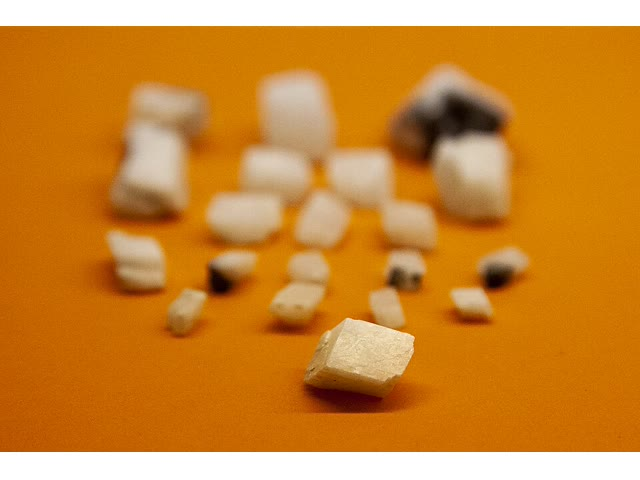
\includegraphics[width=\linewidth]{images/book3/b1-mineral-calcite-rhombs.jpg}

{\scriptsize Romboedros de clivagem da calcita. Fotografia de Giovanna Canu e Eva Santini, CC BY 4.0 (Wikimedia Commons).}
\end{minipage}
\end{inthelab}

\begin{omfigure}
\setlength{\tabcolsep}{2pt}
\begin{tabular}{ccc}
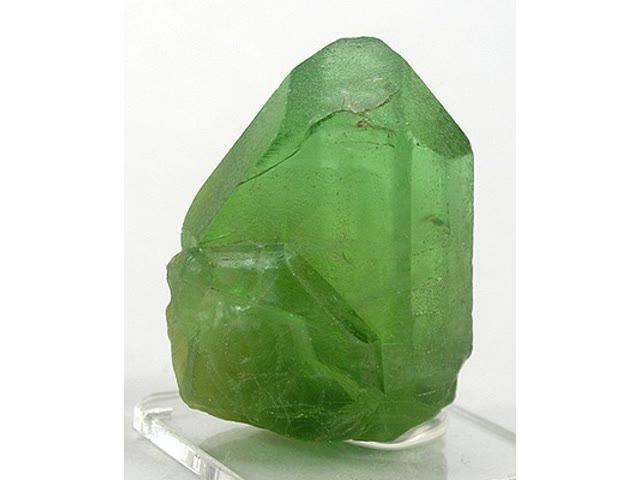
\includegraphics[width=0.31\linewidth]{images/book3/b1-mineral-olivine.jpg} &
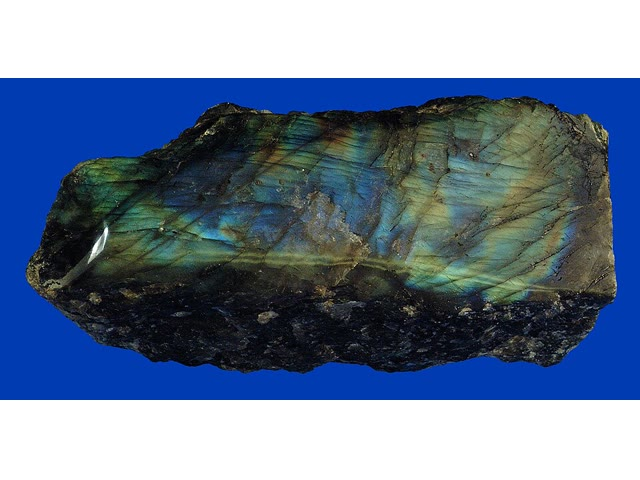
\includegraphics[width=0.31\linewidth]{images/book3/b1-mineral-plagioclase.jpg} &
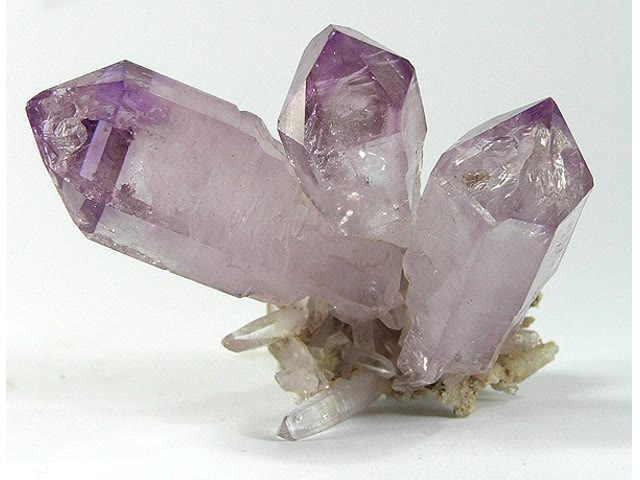
\includegraphics[width=0.31\linewidth]{images/book3/b1-mineral-quartz.jpg} \\
{\small (a) \omterm{def:b1:rock-forming-minerals:groups}{olivina}} & {\small (b) \omterm{def:b1:rock-forming-minerals:groups}{plagioclásio} (labradorita)} & {\small (c) quartzo (ametista)} \\[4pt]
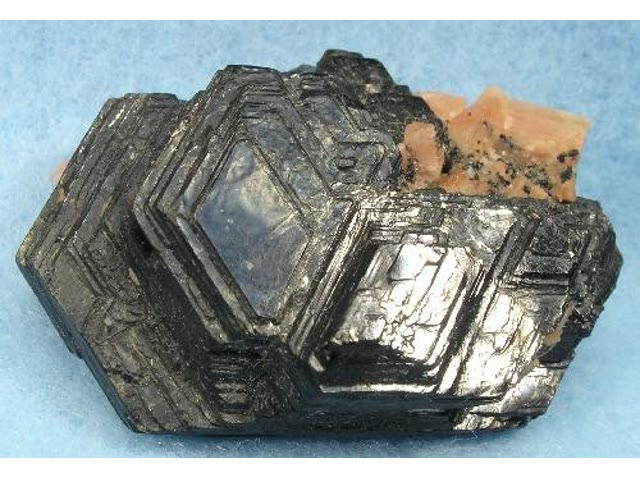
\includegraphics[width=0.31\linewidth]{images/book3/b1-mineral-biotite.jpg} &
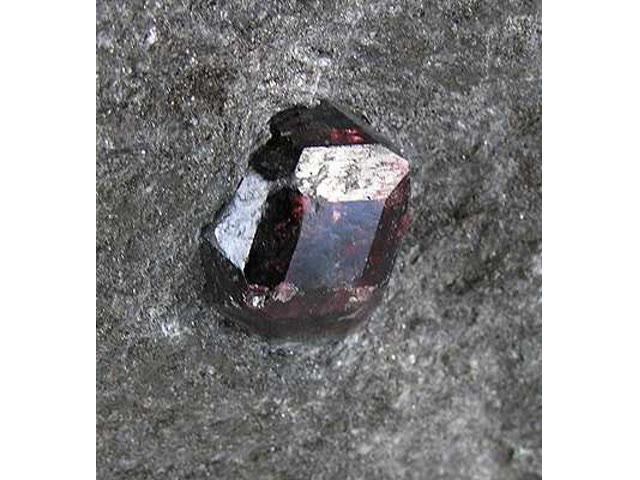
\includegraphics[width=0.31\linewidth]{images/book3/b1-mineral-garnet.jpg} &
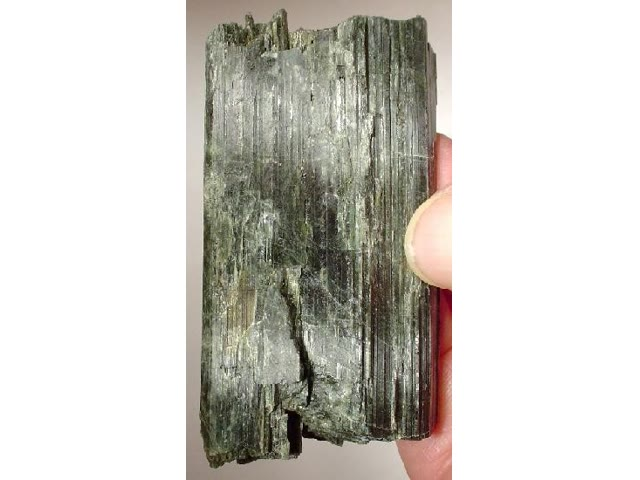
\includegraphics[width=0.31\linewidth]{images/book3/b1-mineral-hornblende.jpg} \\
{\small (d) biotita sobre ortoclásio} & {\small (e) \omterm{def:b1:rock-forming-minerals:groups}{granada} (almandina)} & {\small (f) hornblenda} \\
\end{tabular}
\medskip
% ledger: commons:min-olivine, commons:min-plagioclase, commons:min-quartz, commons:min-biotite, commons:min-garnet, commons:min-hornblende

{\small Seis \omterm{def:b1:rock-forming-minerals:mineral}{minerais} formadores de rochas: (a) um cristal de \omterm{def:b1:rock-forming-minerals:groups}{olivina} de qualidade gema; (b) uma lâmina polida de \omterm{def:b1:rock-forming-minerals:groups}{plagioclásio} mostrando o jogo de cores da labradorita; (c) cristais de quartzo, prismas de seis faces com extremidades piramidais; (d) um livro de lamelas de biotita sobre um cristal de ortoclásio; (e) um cristal de \omterm{def:b1:rock-forming-minerals:groups}{granada} almandina em sua matriz; (f) um prisma de hornblenda. Fotografias (a), (c)--(f) de Robert M.~Lavinsky, CC BY-SA 3.0; (b) de Twyla Baker, CC0 (Wikimedia Commons).}
\end{omfigure}

\section{Exercícios}

\begin{exercise}[$\star$]\label{exo:b1:rock-forming-minerals:1}
Dê o nome da classe de silicato de cada ânion e o número $s$ de vértices compartilhados por cada tetraedro: \ce{SiO4^{4-}}, \ce{Si2O7^{6-}},
\ce{Si6O18^{12-}}, \ce{Si2O5^{2-}}, \ce{SiO2}. A que classe poderia pertencer \ce{SiO3^{2-}}?
\end{exercise}

\begin{exercise}[$\star$]\label{exo:b1:rock-forming-minerals:2}
Com as massas atômicas O \num{15.999}, Si \num{28.085}, Mg \num{24.305} e
Fe \qty{55.845}{g.mol^{-1}}, calcule as massas molares da forsterita e da
fayalita e, depois, os seus volumes molares a partir das densidades \num{3.275} e \qty{4.392}{g.cm^{-3}}.
% ledger: ciaaw:O, ciaaw:Si, ciaaw:Mg, ciaaw:Fe, hom:forsterite, hom:fayalite
\end{exercise}

\begin{exercise}[$\star$]\label{exo:b1:rock-forming-minerals:3}
Em coordenação sêxtupla os raios são \ce{Mg^{2+}} \qty{0.72}{\angstrom},
\ce{Fe^{2+}} \qty{0.78}{\angstrom}, \ce{Ni^{2+}} \qty{0.69}{\angstrom},
\ce{Mn^{2+}} \qty{0.83}{\angstrom} e \ce{Ca^{2+}} \qty{1.00}{\angstrom}.
Calcule a diferença de cada um em relação ao raio do \ce{Mg^{2+}}, em porcentagem, e diga, pelas regras de Goldschmidt, quais podem substituir livremente o magnésio na \omterm{def:b1:rock-forming-minerals:groups}{olivina}.
% ledger: shannon:radii, goldschmidt:size
\end{exercise}

\begin{exercise}[$\star$]\label{exo:b1:rock-forming-minerals:4}
O grafite e o diamante têm densidades \num{2.16} e \qty{3.51}{g.cm^{-3}};
calcita e aragonita, \num{2.71} e \qty{2.93}{g.cm^{-3}}. De quantos por cento a densidade aumenta em cada mudança? Qual \omterm{def:b1:rock-forming-minerals:polymorph}{polimorfo} de cada par se forma sob maior pressão?
% ledger: webmineral:polymorphs, hom:calcite
\end{exercise}

\begin{exercise}[$\star\star$]\label{exo:b1:rock-forming-minerals:5}
Escreva a \omterm{def:b1:rock-forming-minerals:formula}{fórmula estrutural} do \omterm{def:b1:rock-forming-minerals:groups}{plagioclásio} $\text{An}_{30}$ (\qty{30}{\percent}
dos sítios grandes ocupados por cálcio), e confira que ele é neutro.
\end{exercise}

\begin{exercise}[$\star\star$]\label{exo:b1:rock-forming-minerals:6}
Em uma cadeia dupla, metade dos tetraedros compartilha dois vértices e metade compartilha três. Conte os oxigênios de um grupo que se repete de quatro tetraedros diretamente sobre o painel (f) da figura de ligações, e confira a fórmula \ce{Si4O11^{6-}} dada por
\cref{prop:b1:rock-forming-minerals:si-o}.
\end{exercise}

\begin{exercise}[$\star\star$]\label{exo:b1:rock-forming-minerals:7}
Recalcule em quatro oxigênios a análise de \omterm{def:b1:rock-forming-minerals:groups}{olivina} \qty{40.20}{\percent}
\ce{SiO2}, \qty{47.10}{\percent} \ce{MgO}, \qty{12.20}{\percent} \ce{FeO},
\qty{0.40}{\percent} \ce{NiO} (massa molar de \ce{NiO}
\qty{74.692}{g.mol^{-1}}).
Dê a sua \omterm{def:b1:rock-forming-minerals:formula}{fórmula estrutural}, confira-a e dê o seu teor de forsterita. Depois, mostre que o teor de forsterita pode ser encontrado apenas a partir das porcentagens de \ce{MgO} e
\ce{FeO}.
\end{exercise}

\begin{exercise}[$\star\star$]\label{exo:b1:rock-forming-minerals:8}
Confira que a muscovita \ce{KAl2(Si3Al)O10(OH)2} é neutra. Suas folhas de tetraedros têm um alumínio para cada três silícios: que carga isso dá à folha por unidade de fórmula, e qual íon a equilibra?
\end{exercise}

\begin{exercise}[$\star\star$]\label{exo:b1:rock-forming-minerals:9}
Usando os volumes molares \num{42.96} e \qty{46.40}{cm^3.mol^{-1}} e as massas molares \num{140.691} e \qty{203.771}{g.mol^{-1}}: (a) calcule a densidade de $\text{Fo}_{50}$ por mistura ideal, e compare-a com a média das densidades dos \omterm{def:b1:rock-forming-minerals:solid-solution}{membros-finais}; (b) encontre o teor de forsterita de uma \omterm{def:b1:rock-forming-minerals:groups}{olivina} de densidade \qty{3.600}{g.cm^{-3}}.
\end{exercise}

\begin{exercise}[$\star\star\star$]\label{exo:b1:rock-forming-minerals:10}
Com a notação de \cref{prop:b1:rock-forming-minerals:ideal-mixing}, mostre
que
\[
  \rho(x) - \bigl(x\rho_1 + (1 - x)\rho_2\bigr) =
  \frac{x(1 - x)(\rho_1 - \rho_2)(V_1 - V_2)}{V(x)} .
\]
Deduza que a densidade da \omterm{def:b1:rock-forming-minerals:groups}{olivina} fica acima da reta entre os \omterm{def:b1:rock-forming-minerals:solid-solution}{membros-finais}, e calcule a diferença em $\text{Fo}_{50}$.
\end{exercise}

\begin{exercise}[$\star\star\star$]\label{exo:b1:rock-forming-minerals:11}
Um \omterm{def:b1:rock-forming-minerals:groups}{plagioclásio} de um gabro dá \qty{54.10}{\percent} de \ce{SiO2},
\qty{28.90}{\percent} de \ce{Al2O3}, \qty{11.20}{\percent} de \ce{CaO},
\qty{5.10}{\percent} de \ce{Na2O} e \qty{0.30}{\percent} de \ce{K2O} (massas molares \num{60.083}, \num{101.961}, \num{56.077}, \num{61.979},
\qty{94.195}{g.mol^{-1}}). Recalcule-o em oito oxigênios; confira que os sítios tetraédricos (Si + Al) têm 4 átomos e o sítio grande
(Ca + Na + K) tem 1; confira a \omterm{def:b1:rock-forming-minerals:substitution}{substituição acoplada} comparando $\mathrm{Al} - 1$
com Ca; dê o teor de anortita $100\,\mathrm{Ca}/(\mathrm{Ca} +
\mathrm{Na} + \mathrm{K})$.
\end{exercise}

\begin{exercise}[$\star\star\star$]\label{exo:b1:rock-forming-minerals:12}
Uma microssonda não distingue \ce{Fe^{2+}} de \ce{Fe^{3+}} e registra todo o ferro como \ce{FeO}. (a) Mostre que a magnetita pura \ce{Fe3O4}, analisada assim, totaliza \qty{93.09}{\percent}. (b) Recalcule essa análise em quatro oxigênios, e diga por que o resultado é impossível para um \omterm{def:b1:rock-forming-minerals:mineral}{mineral} com três cátions por quatro oxigênios. (c) Recalcule em três cátions, e encontre os números de \ce{Fe^{2+}} e de \ce{Fe^{3+}} exigindo que a fórmula seja neutra. (d) Reexprima a análise como \ce{FeO} e \ce{Fe2O3}, e dê o novo total.
\end{exercise}

\section{Problema: uma olivina de um basalto}

\begin{problem}[{Problema de fim de semana --- recalcular uma análise de microssonda de uma olivina, escrever e conferir a sua fórmula, e encontrar a sua composição, a sua densidade e a sua massa em um metro cúbico de basalto}]
\label{pb:b1:rock-forming-minerals:1}
% invented analysis: figdata/bachelor-1/solid_solution.py (OLIVINE_WT); values: calc/ch07.py
% ledger: ciaaw:O, ciaaw:Si, ciaaw:Mg, ciaaw:Fe, ciaaw:Mn, ciaaw:Ni, ciaaw:Ca, hom:forsterite, hom:fayalite, shannon:radii
Os cristais verdes de um basalto são \omterm{def:b1:rock-forming-minerals:groups}{olivina}. Uma análise de microssonda de um deles
dá, em porcentagem em massa de óxidos:
\begin{center}
\small
\begin{tabular}{lcccccc}
\hline
óxido & \ce{SiO2} & \ce{FeO} & \ce{MnO} & \ce{MgO} & \ce{NiO} & \ce{CaO} \\
massa \% & 39.50 & 16.53 & 0.23 & 43.32 & 0.20 & 0.22 \\
\hline
\end{tabular}
\end{center}
As massas atômicas são O \num{15.999}, Si \num{28.085}, Fe \num{55.845}, Mn
\num{54.938}, Mg \num{24.305}, Ni \num{58.693}, Ca \qty{40.078}{g.mol^{-1}}.
A forsterita tem densidade \qty{3.275}{g.cm^{-3}} e a fayalita
\qty{4.392}{g.cm^{-3}}.

\medskip
\noindent\textbf{Parte I --- Dos óxidos aos cátions.}
\begin{enumerate}
  \item Calcule as massas molares dos seis óxidos.
  \item Calcule o total da análise. O que um total de \qty{97}{\percent} teria sugerido?
  \item Calcule o número de mols de cada óxido em \qty{100}{g} de \omterm{def:b1:rock-forming-minerals:groups}{olivina}.
  \item Calcule os mols de oxigênio que eles contêm, e a sua soma.
  \item Calcule os mols de cada cátion.
  \item Calcule o fator que leva os oxigênios a quatro.
  \item Dê o número de átomos de cada elemento por quatro oxigênios, com três casas decimais.
\end{enumerate}

\medskip
\noindent\textbf{Parte II --- A fórmula estrutural.}
\begin{enumerate}[resume]
  \item A \omterm{def:b1:rock-forming-minerals:groups}{olivina} tem um sítio tetraédrico e dois sítios octaédricos por quatro oxigênios. Calcule a soma dos cátions que não são silício, e compare os dois totais de sítios com a fórmula ideal.
  \item Escreva a \omterm{def:b1:rock-forming-minerals:formula}{fórmula estrutural} da \omterm{def:b1:rock-forming-minerals:groups}{olivina}.
  \item Confira que a fórmula é neutra, e explique por que essa verificação, diferentemente da da questão 8, não poderia ter falhado.
  \item Usando os raios iônicos (\ce{Mg^{2+}} \qty{0.72}{\angstrom}, \ce{Fe^{2+}} \qty{0.78}{\angstrom}, \ce{Ni^{2+}}
        \qty{0.69}{\angstrom}, \ce{Mn^{2+}} \qty{0.83}{\angstrom},
        \ce{Ca^{2+}} \qty{1.00}{\angstrom}, todos em coordenação sêxtupla), explique por que o níquel é comum na \omterm{def:b1:rock-forming-minerals:groups}{olivina} e o cálcio é raro.
  \item A microssonda registra todo o ferro como \ce{FeO}. Explique por que o número total de cátions encontrado na questão 7 mostra que a \omterm{def:b1:rock-forming-minerals:groups}{olivina} não contém \ce{Fe^{3+}} significativo.
\end{enumerate}

\medskip
\noindent\textbf{Parte III --- A composição.}
\begin{enumerate}[resume]
  \item Calcule o teor de forsterita $\mathrm{Fo} = 100\,\mathrm{Mg}/(\mathrm{Mg} +
        \mathrm{Fe})$, com uma casa decimal.
  \item Qual é o \omterm{def:b1:rock-forming-minerals:formula}{número de Mg} da \omterm{def:b1:rock-forming-minerals:groups}{olivina}? Por que ele é igual ao teor de forsterita aqui?
  \item Escreva a \omterm{def:b1:rock-forming-minerals:groups}{olivina} como uma \omterm{def:b1:rock-forming-minerals:solid-solution}{solução sólida} binária
        $\mathrm{Fo}_x\mathrm{Fa}_{1-x}$, ignorando Mn, Ni e Ca, e dê a proporção dos seus sítios octaédricos ocupados por ferro.
  \item Mostre que o teor de forsterita pode ser calculado apenas a partir das porcentagens de \ce{MgO} e \ce{FeO}, sem o fator da questão 6, e faça-o.
  \item Uma \omterm{def:b1:rock-forming-minerals:groups}{olivina} que cresceu depois no mesmo magma tem \qty{40.5}{\percent}
        de \ce{MgO} e \qty{20.0}{\percent} de \ce{FeO}. Calcule o seu teor de forsterita. Qual \omterm{def:b1:rock-forming-minerals:groups}{olivina} é mais rica em ferro?
\end{enumerate}

\medskip
\noindent\textbf{Parte IV --- Densidade e massa.}
\begin{enumerate}[resume]
  \item Calcule as massas molares e os volumes molares da forsterita e da
        fayalita (volumes molares com duas casas decimais).
  \item Tomando a \omterm{def:b1:rock-forming-minerals:groups}{olivina} como a binária $\mathrm{Fo}_x\mathrm{Fa}_{1-x}$ da questão 15, com $x$ arredondado a três casas decimais, calcule a sua massa molar e o seu volume molar por mistura ideal.
  \item Deduza a sua densidade, com três casas decimais.
  \item Compare-a com a interpolação linear entre as densidades dos \omterm{def:b1:rock-forming-minerals:solid-solution}{membros-finais}.
  \item O basalto contém \qty{12}{\percent} de \omterm{def:b1:rock-forming-minerals:groups}{olivina} em volume. Que massa de \omterm{def:b1:rock-forming-minerals:groups}{olivina} contém um metro cúbico do basalto?
  \item O basalto tem densidade de \qty{2.95}{g.cm^{-3}}. Qual é a proporção de \omterm{def:b1:rock-forming-minerals:groups}{olivina} em massa?
  \item Qual é o teor de forsterita da \omterm{def:b1:rock-forming-minerals:groups}{olivina}, arredondado a inteiro por cento?
\end{enumerate}
\end{problem}
